% This is samplepaper.tex, a sample chapter demonstrating the
% LLNCS macro package for Springer Computer Science proceedings;
% Version 2.21 of 2022/01/12
%
\documentclass[runningheads]{llncs}
%
\usepackage[T1]{fontenc}
% T1 fonts will be used to generate the final print and online PDFs,
% so please use T1 fonts in your manuscript whenever possible.
% Other font encondings may result in incorrect characters.
%
\usepackage{graphicx}
\usepackage[table]{xcolor}
\usepackage{booktabs}
\usepackage{orcidlink}
% Used for displaying a sample figure. If possible, figure files should
% be included in EPS format.
%
% If you use the hyperref package, please uncomment the following two lines
% to display URLs in blue roman font according to Springer's eBook style:
%\usepackage{color}
%\renewcommand\UrlFont{\color{blue}\rmfamily}
%\urlstyle{rm}
%
\begin{document}
%
%\title{Automated Eye Opening Detection in Neonates}
\title{Eye opening detection in early neonatal period through CNN}
%
%\titlerunning{Abbreviated paper title}
% If the paper title is too long for the running head, you can set
% an abbreviated paper title here
%
\author{Nuria Velasco-P{\'e}rez\inst{1}\orcidlink{0009-0008-2988-757X} \and 
Juan Arnáez \inst{2}\orcidlink{0000-0001-8883-5181} \and
Nuño Basurto \inst{1}\orcidlink{0000-0001-7289-4689} \and
Daniel Urda \inst{1}\orcidlink{0000-0003-2662-798X}
}
%
\authorrunning{N. Velasco et al.}
% First names are abbreviated in the running head.
% If there are more than two authors, 'et al.' is used.
%
\institute{Grupo de Inteligencia Computacional Aplicada (GICAP), Departamento de Digitalizaci{\'o}n,  Escuela Polit{\'e}cnica Superior, Universidad de Burgos, Av. Cantabria, s/n 09006, Burgos, Spain.\\
\email{\{nuriavp, nbasurto, durda\}@ubu.es} \and
Neonatología, Hospital U. de Burgos. Avda Islas Baleares 3, 09006, Burgos, Spain.}
%
\maketitle              % typeset the header of the contribution
%
\begin{abstract}
Automated detection of neonatal eye opening could support continuous neurological monitoring and facilitate timely clinical interventions in Neonatal Intensive Care Units (NICU). However, this task is challenging owing to unique NICU conditions such as low-contrast lighting, medical device obstructions, and neonates' diminutive facial anatomy. This study explored deep learning approaches for automated neonatal eye state detection by comparing a lightweight CNN architecture trained from scratch with four transfer learning models: VGG16, DenseNet121, ResNet101, and EfficientNetB0. The evaluation was conducted on a carefully curated dataset of 4,119 labeled facial frames extracted from 46 clinical NICU videos. EfficientNetB0 achieved the highest performance with an AU-ROC of 0.928, demonstrating its excellent capability to distinguish between open and closed eyes. The lightweight CNN also yielded competitive results with a significantly shorter training time, highlighting its potential for real-time clinical monitoring. Future research directions include dataset expansion, incorporation of additional facial cues, and application of explainability methods to further enhance clinical interpretability and robustness.
\keywords{Neonatal Monitoring \and Eye Opening \and Deep Learning \and Convolutional Neural Networks \and Transfer Learning}
\end{abstract}
%
\section{Introduction}
\label{sec:introduction}

Monitoring whether a neonate’s eyes are open or closed is clinically relevant for several reasons. First, eye opening is a direct behavioral marker of arousal and responsiveness, routinely scored in neurological examinations such as the \textit{Neonatal Behavioral Assessment Scale} and \textit{Sarnat} staging of hypoxic-ischemic encephalopathy \cite{kurinczuk2010epidemiology}. Second, fluctuations in the eye state correlate with nociceptive responses and the depth of pharmacological sedation, helping clinicians regulate analgesics and avoid pain under- and over-sedation \cite{brown1964states}. Finally, because most life-support equipment in the Neonatal Intensive Care Units (NICU) obscures other facial cues, the eyes remain a comparatively accessible window into the neonate’s neurological integrity \cite{deindl2025eyes}.

Despite its clinical importance, continuous manual observation is impractical in busy NICUs and is subject to considerable inter-observer variability. Vision-based automation offers a promising alternative, enabling objective high-frequency measurements while minimizing handling, a factor known to reduce stress, conserve energy reserves, and promote neurodevelopmental stability.

In recent years, this automation has been increasingly powered by advances in computer vision and Deep Learning (DL), particularly the emergence of pretrained Convolutional Neural Networks (CNN), which have demonstrated strong performance in face detection and landmark localization tasks in adults \cite{niu2020decade}. When integrated into multimodal monitoring systems alongside signals, such as electroencephalography or vital signs, real-time eye state information can enrich early warning systems and support timely neuroprotective interventions \cite{singh2018neo}.

However, neonates present unique challenges: diminutive facial anatomy, variable head posture, medical devices (nasal cannulae, phototherapy goggles), and low-contrast lighting common to incubators. Although domain-specific detectors, such as \textit{NICUface}, have begun to address these constraints, frame-level eye state classification in neonates remains largely unexplored, with existing approaches relying on small datasets and handcrafted heuristics \cite{dosso2022nicuface}.

In this study, an end-to-end framework is presented that first crops the infant’s face with an NICU-adapted detector and then classifies the eye state using two alternative CNN-based strategies: (i) a lightweight model trained from scratch and (ii) a transfer learning baseline. The approach was evaluated using a curated dataset of 4,119 manually annotated frames extracted from 46 clinical videos recorded during routine neurological assessments.

The remainder of this paper is organized as follows: Section \ref{sec:dataset} describes the dataset and the applied preprocessing steps; Section \ref{sec:methodology} presents the proposed classifiers; Section \ref{sec:experimental_design} details the training and evaluation protocol; Section \ref{sec:results} reports and discusses the results; and Section \ref{sec:conclusion} summarizes the main findings and outlines future work.

\section{Dataset}
\label{sec:dataset}

A total of 46 NICU videos were collected from 17 neonates during their first days of life at the \textit{Hospital Universitario de Burgos}. All participants experienced a hypoxic event during birth; the group included both preterm (born between 34 and 36 weeks of gestation) and term infants. Informed consent was obtained from the legal guardians of all participants prior to participation. The recordings underwent the following preprocessing pipeline.


\begin{itemize}

  \item \textbf{Video standardization and clip segmentation.} The original files (\textit{mov}, \textit{avi}, and \textit{mp4}) were converted to \textit{mp4} and split into 400 short clips that isolated distinct clinical stimulations.

  \item \textbf{Frame extraction.} Frames were extracted from each clip at 30 frames per second (fps).
  
  \item \textbf{Face detection}. Faces were located with the MTCNN detector from foundation model called \textit{FaceNet-PyTorch}\footnote{\url{https://github.com/timesler/facenet-pytorch}}, retaining only the highest-confidence bounding box per frame. Frames without valid detection were discarded.
  
  \item \textbf{Temporal down-sampling.} For every 1 second window, the frame with the highest detection confidence was selected, ensuring sharp and centered facial views and reducing redundancy from nearly identical consecutive frames.
  
  \item \textbf{Face cropping and normalization}. The selected bounding box was expanded to a square, resized to 224×224 pixels, and its pixel values were normalized to the mean and standard deviation used for the pretrained models.
  
  \item \textbf{Manual labeling}. Each retained frame was manually categorized as \emph{open} or \emph{closed}. Blurred, occluded, or poorly lit samples were discarded. The resulting dataset contains 4,119 labeled face crops, 3,194 open ($\approx$77\%) and 925 closed ($\approx$23\%), yielding a class ratio of approximately 3.5:1 that is explicitly addressed in the training phase. The distribution is shown in Figure ~\ref{fig:preprocessing_pipeline}.
  
\end{itemize}

\begin{figure}[ht]
    \centering
    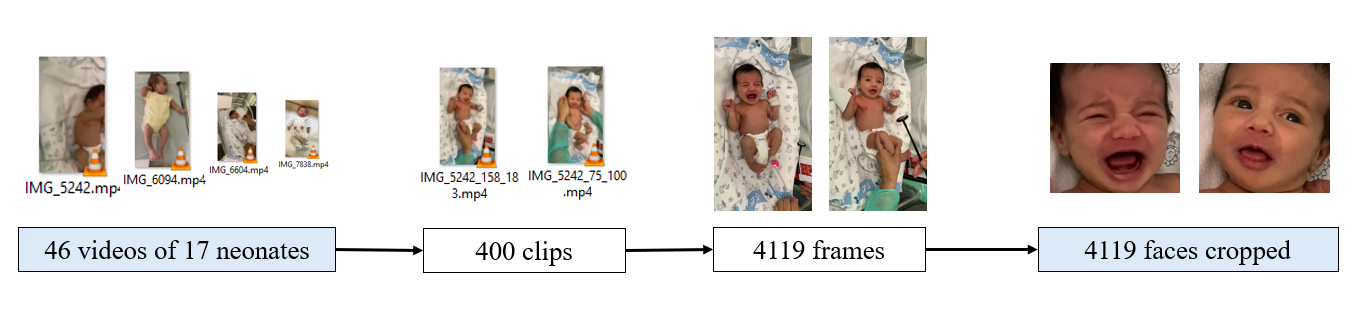
\includegraphics[width=\textwidth]{preprocessing_pipeline.png}
    \caption{Overview of the preprocessing pipeline yielding the 4,119 labeled face crops used for model training and evaluation.}
    \label{fig:preprocessing_pipeline}
\end{figure}

\section{Methodology}
\label{sec:methodology}

A supervised learning approach is employed by leveraging the labeled dataset described in Section~\ref{sec:dataset}. Two complementary CNN-based classification strategies were explored: (i) training a lightweight CNN from scratch, inspired by the classical AlexNet architecture, and (ii) applying transfer learning using several pre-trained state-of-the-art architectures.

\subsection{CNN trained from scratch}

In the first strategy, a lightweight CNN was specifically designed to balance the computational efficiency and classification accuracy. The architecture was loosely inspired by AlexNet, a pioneering deep CNN composed of five convolutional layers followed by three fully connected layers, demonstrating the potential of DL for image recognition tasks \cite{krizhevsky2017imagenet}. Similar to AlexNet, the proposed CNN includes multiple convolutional layers interspersed with max-pooling operations, employs ReLU activation functions, and culminates in fully connected layers for the final classification. However, modifications, such as fewer filters per convolutional layer and reduced fully connected layer dimensions, were introduced to limit the complexity and computational demands, reflecting the smaller scale of the neonatal dataset used in this study.

\subsection{Transfer learning}

Transfer learning leverages the knowledge gained from large-scale datasets (ImageNet in this case) to facilitate training on smaller specialized datasets, thereby reducing the risk of overfitting and significantly accelerating model convergence \cite{tan2018survey}. In this study, four popular pre-trained CNN architectures were evaluated.

\begin{itemize}
    \item \textbf{VGG16}. Known for its simplicity and effectiveness, this architecture consists of 16 convolutional layers using small (3×3) kernels stacked sequentially, followed by max-pooling operations \cite{simonyan2014very}. Although it is computationally demanding owing to its dense layers, it remains a popular baseline for transfer learning due to its robust learned representations.
    
    \item \textbf{DenseNet121}. This is notable for its dense connectivity pattern, where each layer receives input from all preceding layers and passes its outputs to all subsequent layers, thereby significantly alleviating the vanishing gradient problem \cite{huang2017densely}. This architecture efficiently reuses features, requires fewer parameters, and offers competitive performance for various vision tasks.
    
    \item \textbf{ResNet101}. Utilizes residual connections (skip connections) to address degradation problems in deep networks, enabling the stable training of very deep models with 101 layers \cite{he2016deep}. By explicitly modeling residual mappings, ResNet facilitates deeper network architectures without compromising accuracy, thereby leading to improved representational capacity.
    
    \item \textbf{EfficientNetB0}. Introduces a novel compound scaling method that systematically balances depth, width, and input image resolution to enhance accuracy while maintaining low computational requirements \cite{tan2019efficientnet}. EfficientNetB0 is the baseline model of the EfficientNet family and demonstrates high performance in image classification tasks with significantly fewer parameters than traditional CNNs.
\end{itemize}


For each of these pre-trained models, fine-tuning was conducted by initially freezing most of the early convolutional layers (retaining learned low-level features) and retraining only the deeper convolutional and fully connected layers. Importantly, the number of frozen layers was consistent across all transfer learning architectures. This strategy preserved previously acquired generalizable knowledge, adapting only the most specific task-relevant representations for neonatal eye state classification.

\section{Experimental Design}
\label{sec:experimental_design}

\subsection{Training strategy}

The experimental evaluation followed a subject-independent 5-fold cross validation scheme. In each iteration, one fold was reserved for testing, another for validation, and the remaining three were used for training. To prevent data leakage and ensure unbiased evaluation, all frames from the same neonate were consistently assigned to a single fold. In addition, the folds were balanced to maintain approximately similar proportions of \textit{open} and \textit{closed} labels.

All CNN models were trained using the Adam optimizer with a batch size of 64 and an input image size of 224×224 pixels, which is consistent with the standard dimensions established for the pretrained architectures. Early stopping was implemented to monitor the area under the ROC curve (AU-ROC) of the validation set to halt training once the performance plateaued. Binary cross-entropy was selected as the classification loss function. To address the class imbalance, class weights were computed and applied during training, assigning greater importance to the underrepresented (\textit{closed}) class.

Training was conducted using an InfraRed GPU cluster provided by \textit{Junta de Castilla y León}, equipped with 30 NVIDIA Tesla A100 GPUs (40 GB memory each) and delivering a peak computing capacity of 9360 TFLOPS (FP16).

\subsection{Evaluation metrics}

Model performance was assessed using standard classification metrics: accuracy, F1-score, and geometric mean (G-mean). In addition, the areas under the precision-recall (AU-PR) and receiver operating characteristic (AU-ROC) curves were calculated. Accuracy provides overall predictive correctness; F1-score balances precision and recall, reflecting effectiveness in imbalanced settings; and G-mean evaluates balanced predictive performance between classes. AU-PR and AU-ROC further quantify each model's discriminatory ability independent of classification thresholds, which is especially useful in imbalanced scenarios such as this one.



\section{Results and discussion}
\label{sec:results}

Table~\ref{tab:metrics} summarizes the average performance metrics computed over the 5 folds for each tested model, presenting the results from the best-performing hyperparameter configurations. The lightweight CNN trained from scratch demonstrated strong performance, with an AU-ROC of 0.908 and AU-PR of 0.974, achieving a notable accuracy of 0.904 and F1 score of 0.945. Notably, this configuration required only 1.78 minutes of training time, underscoring its computational efficiency and potential suitability for near real-time clinical monitoring.

\begin{table}[ht]
\centering
\renewcommand{\arraystretch}{1.2}
\setlength{\tabcolsep}{4.5pt}
\caption{Performance metrics (Accuracy, F1 score, G-mean, AU-PR, and AU-ROC) averaged over 5 folds for the CNN trained from scratch and four transfer learning architectures. Training times (in minutes) per model are also reported.}
\centering
\begin{tabular}{|l|c|c|c|c|c|}
\hline
\rowcolor{gray!10}
 \textit{Metrics} & \textbf{CNN} & \textbf{DenseNet121} & \textbf{EfficientNetB0} & \textbf{ResNet101} & \textbf{VGG16} \\
\hline
\cellcolor{gray!10} Accuracy   & 0.904 & 0.869 & \textbf{0.908} & 0.876 & 0.891 \\
\cellcolor{gray!10} F1 score   & 0.945 & 0.913 & 0.939 & 0.920 & 0.930 \\
\cellcolor{gray!10} G-mean     & 0.823 & 0.789 & 0.833 & 0.759 & 0.780 \\
\cellcolor{gray!10} AU-PR      & 0.974 & 0.969 & \textbf{0.976} & 0.966 & 0.981 \\
\cellcolor{gray!10} AU-ROC     & 0.908 & 0.905 & \textbf{0.928} & 0.903 & 0.913 \\
\cellcolor{gray!10} Time (min)& \textbf{1.782}  & 14.301 & 15.103 & 13.494 & 14.765 \\
\hline
\end{tabular}
\label{tab:metrics}
\end{table}

Among the transfer learning strategies, EfficientNetB0 yielded the best performance, achieving the highest AU-ROC (0.928) and a notably high AU-PR (0.976). Although the lightweight CNN achieved a marginally higher F1-score (0.945 vs. 0.939), EfficientNetB0 was prioritized because of its superior AU-ROC, the primary metric for imbalanced classification tasks, as it evaluates model performance across all decision thresholds. With an accuracy of 0.908 and a G-mean of 0.833, this model demonstrated a robust ability to effectively classify neonatal eye states, although at the expense of longer training times (15.1 min) than the CNN trained from scratch. 

The remaining transfer learning models (ResNet101, DenseNet121, and VGG16) also exhibited competitive performance, with AU-ROC values consistently above 0.90, G-mean scores of 0.759–0.789, and accuracy of approximately 0.87–0.89, indicating their effectiveness despite slightly lower metrics. Overall, these results illustrate that both lightweight CNNs trained from scratch and pre-trained architectures offer viable approaches for reliable and efficient neonatal eye state detection, with the choice depending on clinical priorities.

\begin{figure}[ht]
    \centering
    \caption{Comparison of the ROC (left) and PR (right) curves for the best performing fold of the chosen model.}
    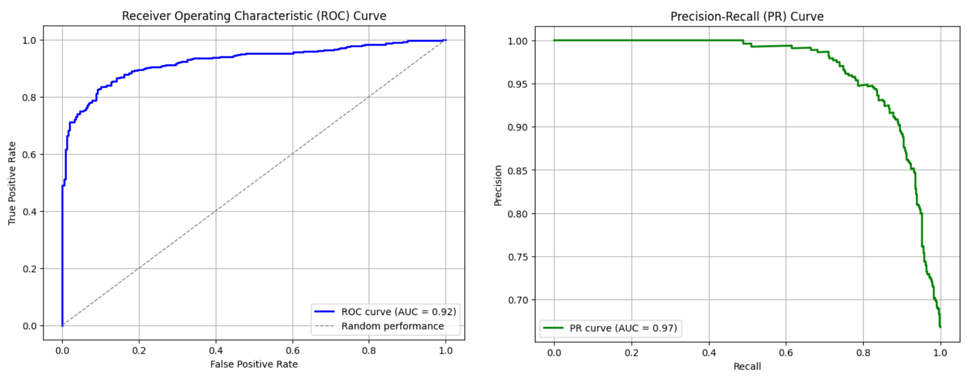
\includegraphics[width=\textwidth]{Plots.PNG}
    \label{fig:au_roc}
\end{figure}

Figure~\ref{fig:au_roc} illustrates the ROC and PR curves for the best-performing fold of EfficientNetB0. The ROC curve reached an AU-ROC of 0.928, indicating excellent discriminative capability across a range of classification thresholds. In addition, the PR curve, with an AU-PR of 0.976, further emphasizes EfficientNetB0’s strong performance under conditions of class imbalance, confirming its robustness as a suitable classifier for this application.

\section{Conclusion and further work}
\label{sec:conclusion}

This study introduced an automated CNN-based pipeline for frame-level classification of neonatal eye state, leveraging face detection and preprocessing specifically tailored to NICU video footage. Among the evaluated models, EfficientNetB0 demonstrated the strongest overall performance, providing an optimal balance between classification accuracy and computational efficiency. The AlexNet inspired CNN trained from scratch also achieved highly competitive results with a significantly reduced training time, highlighting its suitability for real-time deployment in clinical environments.

However, this work has several limitations. First, the class imbalance of the dataset (77\% open-eye frames) may bias the model toward the majority class, despite the use of class weights. Second, all neonates in this study experienced hypoxic events, limiting the generalizability of the results to healthy populations. Finally, the pipeline’s reliance on face detection introduces a potential failure point in cases of extreme head rotation or medical device occlusion.

Future research should focus on expanding the current dataset by incorporating videos from diverse clinical settings and patient populations, thereby enhancing the robustness and generalizability of the model. Extending the existing pipeline to incorporate additional facial cues, such as mouth opening, crying, or facial grimacing, could enable comprehensive multimodal neonatal monitoring and provide a more reliable assessment of neonatal attention and responsiveness. Exploring model explainability techniques, such as Grad-CAM or saliency maps, will also be pursued to identify the regions and visual patterns that influence model predictions, thus improving clinical interpretability and trust in the model. Finally, further hyperparameter optimization and ensemble strategies should be investigated to enhance the prediction consistency and real-time applicability of the system in clinical practice.

Ultimately, the developed CNN-based eye state detection pipeline represents a promising step towards automated, objective, and non-invasive neurological monitoring in NICU environments, potentially improving neonatal clinical outcomes through earlier interventions and more precise care.
% ---- Bibliography ----
%
% BibTeX users should specify bibliography style 'splncs04'.
% References will then be sorted and formatted in the correct style.
%
% \bibliographystyle{splncs04}
% \bibliography{mybibliography}
%
\begin{thebibliography}{8}
\bibitem{kurinczuk2010epidemiology}
Kurinczuk, J.J., White-Koning, M., Badawi, N.: Epidemiology of neonatal encephalopathy and hypoxic-ischemic encephalopathy. Early Human Development, 86(6), 329--338 (2010)

\bibitem{brown1964states}
Brown, J. L. States in newborn infants
Merrill-Palmer Quarterly of Behavior and Development, 10(4), 313--327 (1964).

\bibitem{deindl2025eyes}
Deindl, P., Luister, A., Vettorazzi, E., Pointner, N., Singer, D., Berger, A., Wagner, M., Giordano, V.: Eyes on Newborns: How NICU Staff's Attention and Emotions Shape Neonatal Pain Assessment. European Journal of Pain, 29(3), e4791 (2025)

\bibitem{dosso2022nicuface}
Dosso, Y. S. Kyrollos, K. J. Greenwood, J. Harrold, and J. Green, J. R.
\textit{NICUface: Robust neonatal face detection in complex NICU scenes}.
IEEE Access, 10, 62893--62909 (2022).

\bibitem{niu2020decade}
Niu, S., Liu, Y., Wang, J., \& Song, H.
\textit{A decade survey of transfer learning (2010--2020)}.
IEEE Transactions on Artificial Intelligence, 1(2), 151--166 (2020).

\bibitem{singh2018neo}
Singh, H., Kaur, R., Gangadharan, A., Pandey, A.K., Manur, A., Sun, Y., Saluja, S., Gupta, S., Palma, J.P., Kumar, P.: Neo-bedside monitoring device for integrated neonatal intensive care unit (iNICU). IEEE Access, 7, 7803–7813 (2018)

\bibitem{krizhevsky2017imagenet}
Krizhevsky, A., Sutskever, I., Hinton, G.E.: ImageNet classification with deep convolutional neural networks. Communications of the ACM, 60(6), 84–90 (2017)

\bibitem{tan2018survey}
Tan, C., Sun, F., Kong, T., Zhang, W., Yang, C., Liu, C.: A Survey on Deep Transfer Learning. In: Kůrková, V., Manolopoulos, Y., Hammer, B., Iliadis, L., Maglogiannis, I. (eds) Artificial Neural Networks and Machine Learning – ICANN 2018. Lecture Notes in Computer Science, vol 11141, pp. 270–279. Springer, Cham (2018). https://doi.org/10.1007/978-3-030-01424-7\_27

\bibitem{simonyan2014very}
Simonyan, K., Zisserman, A.: Very deep convolutional networks for large-scale image recognition. arXiv preprint arXiv:1409.1556 (2014)

\bibitem{huang2017densely}
Huang, G., Liu, Z., Van Der Maaten, L., Weinberger, K.Q.: Densely connected convolutional networks. In: Proceedings of the IEEE Conference on Computer Vision and Pattern Recognition, pp. 4700–4708 (2017)

\bibitem{he2016deep}
He, K., Zhang, X., Ren, S., Sun, J.: Deep residual learning for image recognition. In: Proceedings of the IEEE Conference on Computer Vision and Pattern Recognition, pp. 770–778 (2016)

\bibitem{tan2019efficientnet}
Tan, M., Le, Q. EfficientNet: Rethinking model scaling for convolutional neural networks. In: International Conference on Machine Learning, pp. 6105–6114, PMLR (2019)

\end{thebibliography}
\end{document}
